% General comments / corrections:
% - be consistent in use of "B" vs "B molecules"
%
\section{Introduction}
\label{sec:Introduction}
% - carbon blacks instead of soot (materials focus)

%% Curved carbons are everywhere...
Curved carbons are found in many materials including porous carbons, glassy carbons, activated carbons~\cite{Harris2005new,Martin2019topology,Martin2019nanostructure} and soot particles~\cite{Martin2018flexo}. For example, high resolution transmission electron microscopy of energy-relevant carbon materials such as coke and soot, shows that a significant proportion (63\% for young particles, 28-49\% for mature carbons) of the constituent molecules are curved \cite{wang2017improved,zhong2018structural,Martin2018flexo}. 
Curved carbon molecules have many different names including bowl-shaped compounds, buckybowls, $\pi$-bowls, fullerene-like fragments. In this work we will refer to them as curved polycyclic aromatic hydrocarbons (cPAHs), since flat polycyclic aromatic hydrocarbons (fPAHs) will be used as a comparison.

%% Curvature is caused by, properties 
Curvature is predominantly caused by the presence of non-hexagonal rings, such as pentagons, within a hexagonal lattice~\cite{Martin2018polar}. The resulting molecules have steric and electronic properties not present in defect-free carbon materials containing hexagonal structures only. In particular, the curvature redistributes electronic charge in the $\pi$-cloud and causes the molecules to possess a dipole moment due to the flexoelectric effect~\cite{Martin2017}. This allows curved molecules to interact in long-range electrostatic interactions, not present in systems containing planar carbon molecules. However, these molecules retain aromaticity and show considerable electron delocalisation \cite{grabowsky2010electron,Dobrowolski2011aromatic}.

%% curved carbon applications...
These qualities cause the presence of curved aromatic molecules to influence material structure and properties. Curved molecules increase material porosity \cite{Harris2005new} and facilitate stronger adsorbate-adsorbent interactions \cite{Martin2017}, which combined with high polarisability and high surface area provide enhanced adsorption important for applications such as carbon sequestration, gas storage and separation~\cite{Scanlon2006investigation}.

Curved aromatics also possess a combination of properties, including surface charge stabilisation, high charge mobility, significant dipole moment, and small band gap~\cite{Menon2019optical}, that make them excellent candidates for applications such as optoelectronic devices, organic semiconductors, liquid crystals, electrodes, imaging probes, and batteries. For example, integrating corannulene inside insulating porous scaffolds allows electronic properties to be tuned and results in a 10,000-fold conductivity enhancement \cite{rice2018stack}. Flame-formed carbon nanoparticles show quantum dot behaviour \cite{liu2019flame}, which have shown great promise in bioimaging, photovoltaic and light emitting applications due to their biocompatibility, luminosity, and solubility \cite{zhang2012graphene}.
% Good promise in electronics applications because of tunable optoelectronic properties \cite{sanyal2014functional}
% suggested for sensors and molecular machines (10.1039/c6cp05841h)

The alignment of columnar or stacked structures is important for mechanical and electronic properties of materials, and for the generation of graphisiting material. In some cases the presence of curved molecules contributes to a low degree of molecular ordering in a material %and poor stacking (only ~20\% stacked)
\cite{zhong2018structural} and may prevent graphitisation by disrupting the formation of the mesophase. For example, the integration of curvature in molecules is crucial in determining whether a carbonised material produces graphitic or non-graphitised carbon \cite{abrahamson2018carbon}. Columns of cPAHs also show high electron transport characteristics desirable for high-performance materials for organic electron devices \cite{wang2015electronic}.

Accurately describing and characterising the structure and self-assembly of curved carbon materials is of interest to production processes since curvature is easily integrated as a defect (more stable than planar). This is crucial for understanding many ubiquitous materials, such as combustion-produced particles and graphite from mesophase pitch.
%
%Carbon materials have been fabricated for use as adsorbents, carriers, catalyst supports, electrodes, and other advanced applications (refs).  The performance of these materials can be directly improved/tuned for these applications by adjusting their physical properties - in particular their nanostructures.  It is therefore crucial to develop a detailed understanding of the molecular interactions involved to enhance the prediction and design of desired carbon nanostructures.

In addition to providing the understanding required to optimise the nanostructures for these applications, this provides insight into the natural processes and environments that generate nanoparticles containing polycyclic aromatic hydrocarbons, such as combustion-produced pollutants~\cite{Martin2018flexo} and interstellar medium~\cite{Lovas2005}.

%% Previous work looking at cPAH interactions:	Homogeneous dimers; Pi-pi > pi-CH interactions, eclipsed > staggered.
Previous work on the structure and properties of polycyclic aromatic hydrocarbons has focused on fPAHs~\cite{Grancic2016,chen2014size,Rapacioli2005stacked,hernandez2017dynamics}, with less attention given to cPAHs. Electronic structure calculations show that there are significant interactions between nested concave-to-convex homogeneous cPAH dimers, and their curvature does not prevent dimers from forming $\pi$-$\pi$ stacked assemblies similar to planar systems~\cite{sygula2009pi,Cabaleiro-Lago2018}. As with fPAHs, cPAH dimer interactions are dominated by $\pi$-$\pi$ interactions compared to CH-$\pi$ interactions. However cPAHs in the concave-convex dimer configuration show different behaviour than fPAH dimers and cPAHs in convex-convex configuration, with the eclipsed dimer (in which the aromatic planes are aligned) showing a higher stability than the staggered dimer (in which the aromatic planes are shifted relative to each other)~\cite{janowski2011convex,Cabaleiro-Lago2018}.
Dispersion provides the dominant energy contribution, although electrostatics are also significant especially in contrast to fPAH dimers, due to the permanent dipole moment~\cite{Cabaleiro-Lago2018,janowski2011convex}.

Different degrees of curvature can result in increased or decreased cPAH dimer strengths, due to geometry and electrostatic effects. Curvature is able to increase interaction strength by decreasing C-C distances for increased dispersion interactions \cite{kennedy2012buckyplates}. 
%However, very curved PAHs have lower interaction strengths similar to fPAHs due to increased steric hinderance (10.1016/j.proci.2018.05.046, \cite{sygula2009pi}). High curvature also increases exchange-repulsion and can destabilise the dimer (\cite{kennedy2012buckyplates}, \cite{sygula2009pi}).

%% Previous work looking at cPAH interactions:	Bulk systems
X-ray and density functional theory calculations have shown that the crystal structure of cPAH systems are determined by an interplay of electrostatic and dispersive forces, but predicting the packed structure of cPAHs is not straightforward. The dipole moment and molecule bowl depth are identified as significant factors, but do not have clear threshold values that guarantee particular molecular arrangements \cite{Filatov2010}. In addition, the size, curvature, rigidity, functionalisation, and atomic composition of cPAHs are known to influence their ability to form columnar stacks in solid state \cite{wang2015electronic,scott1999geodesic,grabowsky2010electron,sygula1994bowl,bronstein2002practical,forkey1997crystallographic,roch2017indenocorannulene,petrukhina2004hemibuckminsterfullerene,petrukhina2005unprecedented,Filatov2010,sakurai2005structural,imamura1999triphenyleno,wu2006aromatic,sanyal2014functional}. These systems show large $\pi$-$\pi$ overlap and staggered stacked interactions to produce extended $\pi$ networks enhanced by CH-$\pi$ interactions.

%% Previous work looking at cPAH interactions:	Heterogeneous systems (dimers, etc)
% TO DO: make this paragraph more clear by splitting ideas: increased electrostatics and interactions with ions vs different structure and bowl complementarity
Computational studies of fPAHs show that, unlike cPAHs, heterogeneous dimers are significantly weaker than their homogeneous counterparts (ref). This heterogeneity decreases the stability of a nanoparticle containing different molecule sizes and leads to a distinct partitioning in which the larger molecules formed the cluster core and the smaller molecules resided in the outer shell \cite{bowal2018partitioning}. Dynamic interactions of cPAHs or fPAHs with cations also highlight the ability of cPAHs to engage in electrostatic interactions that stabilise a cPAH cluster, while fPAHs cannot \cite{bowal2019ion}. These results suggest that the fundamental interaction differences between fPAHs and cPAHs may cause different clustering and packing behaviours. Preliminary work suggests that the nanostructure of homogeneous cPAH clusters is significantly different from similar-sized fPAH clusters \cite{bowal2019ion}, and perhaps different molecule sizes will show increased packing and stability due to bowl complementarity.
% This may be more representative of the experimentally observed structure of nascent soot particles.

%So expect homogeneous corannulene nanocluster to be disordered, homo 2pent15ring cluster to have stacks. Expect mixed cPAH cluster to be dominated by 2pent15rings but enhanced corannulene stacking and more stable than comparable mixed fPAH cluster.
% cPAH interactions with different sized molecules (no heteroatoms) (refs????). Increased stability compared to heterogeneous fPAH systems because of shape fitting and enhanced electrostatics and CH-pi interactions (?).
%Homodimers are weaker than heterodimers because they don't take advantage of bowl complementarity (\cite{Cabaleiro-Lago2018}).
%Thus we hypothesise that heterogeneous cPAH clusters may be more stable than their heterogeneous fPAH counterparts since different sizes of cPAHs may provide stable packing arrangements.
%

%% Limitations of existing work
To date detailed studies of cPAHs have primarily included static DFT calculations or crystal structure experiments, as described above, neither of which provide information about intermolecular dynamics and particle nanostructure.
%
%% purpose of this work... 
%The structural properties of cPAH clusters are unknown and further molecular modelling studies are required to provide insight into the clustering behaviour of cPAHs - their size-dependent arrangements in both homogeneous and heterogeneous systems, interactions with planar PAHs, and assembly around ions. Understanding non-covalent interactions with and between curved carbon nanostructures has importance in many systems and great potential for numerous applications.
% Development requires understanding of self-assembly and dynamic nanostructure of curved aromatics
%
The purpose of this work is to explore properties of clusters containing cPAHs, with the aim of answering the following questions: 

%What is the energy and structure of cPAH nanoparticle systems and how do these differ from systems containing fPAHs? What is the influence of molecule size, proportion, and presence of ions or fPAHs? 
This is done by extending a force field for complex cPAH systems and using this within molecular dynamics to provide a detailed assessment of cPAH cluster self-assembly.
%with the aim of answering the following questions: Are cPAH clusters more stable than fPAH clusters? Do cPAHs partition within clusters the same way fPAHs do? What is the internal nanostructure and surface composition of cPAH particles?  
%In this work, we are motivated to understand the influence of cPAHs in soot particle structure and stability, but these results have general relevance to nanoparticles containing cPAHs regardless of source or application.
%Hypothesis: cPAH clusters are more representative of the experimentally observed structure of nascent soot particles, heterogeneous cPAH clusters are significant since they are stable than their fPAH counterparts.
These are important for better understanding carbon nanomaterial applications such as batteries, imaging probes, gas storage, optoelectronics, and targeted nanomedicine.
We address these questions by studying nanoparticle systems containing cPAHs, first in homogeneous clusters containing one molecule type only, then extending this to heterogeneous clusters to understand the interactions and effect of cPAH size and ratio. Finally, exploratory work on heterogeneous systems containing cations or fPAHs is presented. %% TO DO: change this so not giving homo, hetero, etc in a particular sequence

%%%%%%%%%%%%%% Other notes to perhaps include %%%%%%%%%%%%%
% Functionalisation allows stacking solid-state structure in corannulene systems (chemical nature and position of functional groups strongly affects the stacking geometry) which influence optoelectronic properties \cite{sanyal2014functional,mack2007development}.
% "Properties of a matter are intrinsically dependent on the internal arrangement of molecules in the solid state. Therefore, knowledge of three-dimensional structure of the matter is a prerequisite for structure–property correlations and design of functional materials. Over the past century, X-ray crystallography has evolved as a method of choice for accurate determination of molecular structure at atomic resolution. The structural information obtained from crystallographic analysis paved the way for rapid development in electronic devices, mineralogy, geosciences, materials science, pharmaceuticals, etc."


\section{Methods}
\subsection{Force field development}
The isoPAHAP potential is an all-atom isotropic intermolecular description developed for fPAHs~\cite{totton2010first}. It shows good agreement with high accuracy quantum calculations and has been used in dynamic and stochastic simulations of fPAH systems~\cite{Totton2012quantitative,bowal2019sphere,Grancic2016,Pascazio2017}. This potential uses fixed atom-centred charges, which are suitable for fPAHs where electrostatic interactions arise principally from the terminal groups. It is not able to capture local dipole moments located at strained internal carbon sites within curved PAHs. Therefore we previously developed a new atomic potential for cPAHs, called the curPAHIP potential~\cite{bowal2019ion}. The curPAHIP potential models the increased polarity of cPAHs using a modified molecule description with off-site point charges located above the pentagonal carbon atoms and optimised potential parameters parameterised to SAPT(DFT) energies.

To accurately model the flexoelectric dipole moment within this potential, we extend the molecular description to include larger cPAHs and assessed the suitability of the curPAHIP potential. Following the parameterisation method developed for A in \citet{bowal2019ion}, B is minimised and mass-less charges are added 0.052~nm above each of the pentagonal carbon atoms to match the calculated dipole moment of 5.28~D~\cite{Martin2018flexo}. The resulting atomic coordinates and charges of the minimised B monomer (as well as A) are provided in the Supplementary Information Section~\ref{sec:SImoleculedesc}.

The binding energies of cPAH dimers are calculated to assess the suitability of curPAHIP in describing systems containing larger cPAHs. Density functional theory (DFT) calculations are used to determine the geometry of cPAH monomers and geometries and energies of cPAH dimers using a methodology similar to that used by \citet{Martin2018polar} (see Supplementary Information Section~\ref{secSI:DFT} for details). Binding energies are shown for four dimer types in Figure~\ref{fig:potentialDFTcurves}. The energy of the isoPAHAP potential is also included to highlight the behaviour of a fPAH potential that does not include the enhanced electrostatics and dispersion due to the flexoelectric effect and increased polarisability, respectively, and in all cases the isoPAHAP potential significantly underestimates the binding energy and overestimates the equilibrium dimer distance.
The curPAHIP potential agrees very well with the DFT and SAPT(DFT) results for the A dimer, Figure~\ref{fig:potentialDFTcurves}(a). This is expected since these \textit{ab~initio} values were used in the parameterisation of the curPAHIP potential~\cite{bowal2019ion}. 
Figure~\ref{fig:potentialDFTcurves}(b) shows that the curPAHIP potential can be extended to cPAH molecules larger than A, since there is good agreement (within 5\% of the dispersion-corrected DFT energies) for the larger B. In contrast, the isoPAHAP gives a minimum energy value that is 31\% smaller than the DFT calculations.
The energies of heterogeneous dimers, containing one A and one B, are also well captured by the curPAHIP potential, as seen in Figure~\ref{fig:potentialDFTcurves}(c) and (d). The repulsive branch of the curPAHIP potential is slightly shifted to smaller distances than the DFT values in some cases, which is acceptable since the repulsive branch has been shown to weakly influence PAH cluster formation with the interaction well depth playing the significant role~\cite{Pascazio2017}. Of note, the nested dimer with the smaller A on the concave side of the larger B (Figure~\ref{fig:potentialDFTcurves}(c)) shows a T-shaped type configuration. In this system the curPAHIP potential provides a slightly smaller %need to quantify? 
angle between the two molecules in the minimum energy configuration than the DFT calculation, suggesting that CH-$\pi$ interactions are weaker and $\pi$-$\pi$ overlap is favoured using the intermolecular potential.  This difference does not seem to cause a significant difference in larger systems, however, as discussed further in the alignment angle analysis. 
%
\begin{figure}[!tbh]
\centering
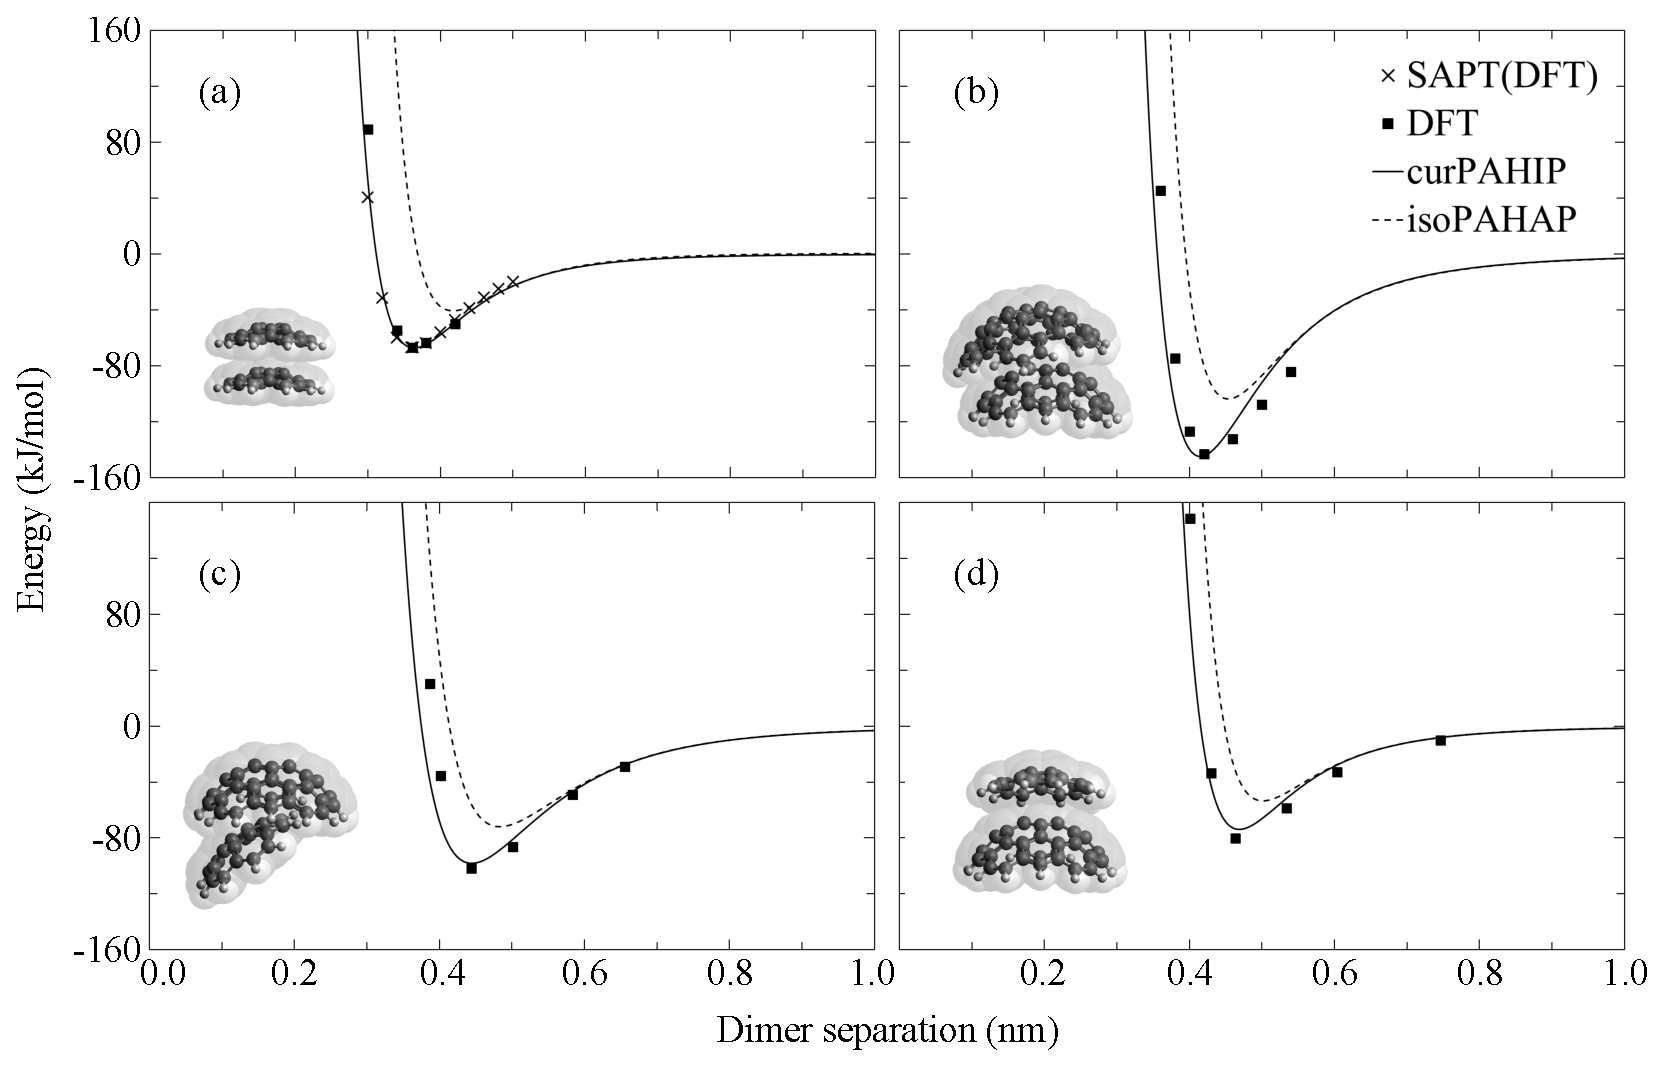
\includegraphics[width=1\linewidth]{Figures/potentialDFT_curves.eps}
\caption{Interaction energy versus separation distance for cPAH dimers determined from SAPT(DFT) calculations~\cite{Cabaleiro-Lago2018}, DFT calculations, the curPAHIP potential, and the isoPAHAP potential. The dimers are as follows: (a) two A, (b) two B, (c) and (d) one A and one B each.}
\label{fig:potentialDFTcurves}
\end{figure}
%

Further details on the isoPAHAP and curPAHIP potential forms and parameters are found in the Supplementary Information Section~\ref{sec:SIpotentials}. For simulations considering both fPAHs and cPAHs in a single cluster, the curPAHIP potential was used to describe the mixed molecule interactions and simulations using the isoPAHAP potential to describe these interactions show very similar results.

%%%%%%%%% perhaps to add to discussion:
% Overall some slight differences compared to DFT results show repulsive component of curPAHIP is shifted to smaller distances (means that there might be stronger attractions at small dimer separation distances) and minimum is slightly lower energy (provides conservative case if any different (less likely to bond))
% The difference between the DFT and curPAHIP energies can be partly explained by the fact that the MD minimised monomers (used in curPAHIP assessment) are more curved than the DFT monomers. So perhaps the energies are not as low for the curPAHIP potential since the dimers are not able to reach the same small distance values without steric hindrance and repulsion coming into effect.

\subsection{Systems} %% systems studied
To thoroughly evaluate the self-assembly of nanoparticles containing cPAHs, three different molecule types with different sizes and degrees of curvature are considered: coronene (\ce{C24H12}), a small fPAH containing seven hexagons, corannulene (\ce{C20H10}), the smallest cPAH containing one central pentagon with five surrounding hexagonal rings, and \ce{C42H14}, a larger cPAH containing two embedded pentagons, all shown in Figure~\ref{fig:clustersnapshots}. The notation $\text{X}_{\text{y}}$ is used to describe the clusters studied, where X values refer to the molecule types and y gives the number of each type of molecule within the cluster. The molecule species considered in this work are: corannulene (indicated as A), \ce{C42H14} (B), coronene (fPAH \ce{C24H12}) (C), circumcoronene (fPAH \ce{C54H18}) (D), and potassium cation (K). For example, $\text{A}_{\text{50}}\text{B}_{\text{50}}$ indicates a cluster containing 100 molecules, made up of 50 corannulene and 50 \ce{C42H14} molecules.

%% TO DO: change the wording of this section so not sequential through different cluster types! Also use the naming notation to make this section less wordy?
The influence of particle size, molecule size, molecule ratio, and ion interactions, are evaluated by considering 17 different clusters. First, homogeneous clusters containing 25, 50, 100, and 200 A and clusters containing 25, 50, and 100 B are studied to provide information across molecule and cluster sizes. 
Second, a series of binary clusters each containing 40 molecules of different sizes and proportions allows evaluation of heterogeneity effects. Heterogeneous clusters containing A and B in proportions of 40:0, 30:10, 20:20, 10:30, and 0:40 are studied. In addition, a heterogeneous cluster containing 50 A and 50 B addresses heterogeneous cluster size effects.
Third, clusters containing 20 A and 20 C provide insight into the interactions between cPAHs and fPAHs.
Finally, clusters containing 40 A or B with one or two potassium cations allow investigation into the self-assembly of ion-containing clusters.
Snapshot images of each cluster considered in this work are shown in Figure~\ref{fig:clustersnapshots}. We should note that in this work, the terms (nano)particle and cluster are effectively synonymous: a nanoparticle is a cluster of molecules.

Four clusters containing both A and B are examined to understand the self-assembly of heterogeneous cPAH clusters. The $\text{A}_{\text{10}}\text{B}_{\text{30}}$, $\text{A}_{\text{20}}\text{B}_{\text{20}}$, and  $\text{A}_{\text{30}}\text{B}_{\text{10}}$ clusters show the influence of molecular ratio, and the $\text{A}_{\text{50}}\text{B}_{\text{50}}$ cluster highlights influences due to cluster size. 

\subsection{Molecular dynamics}
Equilibrium cluster configurations are produced using a multi-step molecular dynamics simulation process. Clusters are initialised in a mixed configuration, with molecules randomly placed within a large spherical volume using the PACKMOL software \cite{Martinez2009PACKMOL}. Excess energy is removed by an energy minimisation step using the steepest descent algorithm, followed by the low-memory Broyden-Fletcher-Goldfarb-Shanno method \cite{L-BFGS}.

Replica Exchange Molecular Dynamics (REMD) simulations are used to rapidly produce equilibrated cluster systems. Modelled after Monte Carlo parallel tempering \cite{Hukushima1996}, REMD is an advanced form of molecular dynamics that involves evaluating simultaneous isothermal systems, called replicas, across a temperature range \cite{Sugita1999}. At regular intervals throughout the simulation, neighbouring replicas are able to exchange spatial information based on a Boltzmann-weighted temperature dependent probability. This method allows efficient sampling of the system potential energy since low energy replicas are able to explore new configurations generated by higher energy replicas. 
% REMD simulations use a large number of interacting parallel simulations to rapidly determine stable structures across a large range of temperatures.
% able to rapidly determine low energy configurations by using higher energy parallel systems to explore new arrangements. % REMD was developed to enhance sampling of a complex potential energy surface, based on the fact that the rate at which barrier-crossing events occur is increased with an increase in temperature. 
% As a result, after an exchange, each low energy configuration exchanged into a higher energy replica has a better opportunity to overcome energy barriers and move into a new lower energy region of phase space, while each swapped high energy configuration provides a low energy replica with a fresh configuration to sample. 

In this work, REMD simulations are conducted for 3~ns. A large temperature range is selected to include solid-like and liquid-like particle morphologies. For clusters containing A, B, A and B, and A and C this corresponds to temperature ranges of 200--800 K, 400--1600 K, 200--1600 K, 200--800 K, respectively. These require between 27 and 84 REMD replicas to maintain an acceptable replica exchange acceptance. Further information detailing the replica temperature selection and an assessment of effectiveness is given in the Supplementary Information Section~\ref{secSI:REMDtemps}. As described in detail in similar work~\cite{bowal2018partitioning}, a flat-bottomed spherical position potential is applied within the REMD simulations to address complete evaporation of small molecules from the cluster at high temperatures. Individual 1~ns simulations using classical molecular dynamics (MD) are then conducted at each desired temperature from the final REMD configurations. No position potential is implemented for these post-REMD MD simulations.

In the REMD and MD simulations the NVT ensemble, where a constant number of atoms, system volume, and temperature are maintained, is sampled using chain of $10$~Nos\'{e}-Hoover thermostats for temperature control. A velocity Verlet integrator~\cite{Verlet_1967} is used to advance the configuration in 1~fs time steps and all simulations are conducted \textit{in vacuo} without periodic boundary conditions.  Intramolecular forces are determined using the OPLS-AA force field~\cite{Kaminski2001opls} for molecular bonds, angles, dihedral and improper dihedral angles. The curPAHIP intermolecular potential~\cite{bowal2019ion}, parameterised for cPAHs and discussed in more detail in the following section, is used to describe interactions between cPAHs and intermolecular cut-offs are set to $3.0$~nm. All minimisation, REMD, and MD simulations are conducted using GROMACS~5.1.4~\cite{Abraham2015}. Purpose-made scripts are used to the process the output and VMD~\cite{Humphrey1996} provides visualisations.


%%%%% Analyses %%%%%
\subsection{Structural analyses}
% Structural analysis - Molecular arrangement analysis (radial distances, coordination numbers, stacking angle, etc).
A number of different metrics, including intermolecular spacing, coordination number, alignment angle, and radial distance, are used to evaluate system structural properties. All metrics are averaged over the final 500~ps of the post-REMD simulation of the lowest temperature replica (\textit{i}.\textit{e}. 3500--4000~ps of total simulation time) using a timestep of 1~ps. 
%The final 500 ps of the post-REMD MD simulations are equilibrated and show <5\% drift in energy so this was selected as the production period.
Many calculations require the identification of near neighbours for each molecule within the system. For this, molecule centres of mass and the cut-off radius $R$ are used. Molecules are considered neighbouring if their centres of mass are within the cut-off radius for at least half of the 500~ps production period. Unless otherwise stated, values of $R$ are selected to allow $>85\%$ of molecules to have at least one identified neighbour. This results in cut-off radii of $R_{\text{A}} = 0.7$~nm, $R_{\text{B}} = 0.5$~nm, and $R_{\text{C}} = 0.5$~nm for A, B, and C, respectively. 
% These cut-off radius values are used for both homogeneous and heterogeneous clusters 
%Although it may seem counter-intuitive that the smaller cPAH uses the larger cut-off distance, this is due to the different interaction types of the two molecules which will be discussed later.

%Intermolecular spacings are calculated between each molecule and its neighbours within $R$ and averaged over all equilibrated timesteps. The reported values are averaged over molecule type interactions in the system, including: all, B-B, A-A, and B-A.

% alignment angles
Molecular alignment angles are calculated to provide information on the relative configurations of neighbouring molecules within the clusters studied. An alignment angle is defined as the angle between normal vectors to the central rings (for A this is the pentagonal ring and for B this is the central hexagonal ring) of the neighbouring cPAHs considered.  Figure~\ref{fig:alignmentangles_homo} provides a schematic of the alignment angle between two neighbouring A.

% coordination numbers
A quantitative measure of the degree of stacking order in the molecular structures is provided through the use of coordination numbers (CNs), calculated as the number of near neighbours averaged over each molecule type. To consider only $\pi$-$\pi$ stacking interactions within this metric, values of $R$ are selected to include sandwich-type stacked interactions between molecules but exclude molecules more than one layer away. Equilibrium dimer distances provide the minimum $R$ values for each molecule type as $R_{\text{A}} = 0.4$ nm and $R_{\text{B}} = 0.5$~nm.

% radial distances
Radial distances are defined as the distance between a molecule type and the cluster centre averaged over all atoms and provide insight into the spatial partitioning of molecule types within a cluster, particularly useful for understanding the self-assembly of heterogeneous systems.

The sensitivity of the cut-off values on calculated cluster properties is discussed in the Supplementary Information Section~\ref{secSI:cutoffs}. Further information on the calculation of the radial distances and coordination numbers is also provided in the Supplementary Information Section~\ref{secSI:raddist_CN_eqns}.

%These metrics were assessed and represent the A crystal structure well (see Supplementary Information Section~\ref{secSI:corannulenecrystal} for more details).


\section{Results and Discussion}
%
Figure~\ref{fig:clustersnapshots} shows all of the low energy cluster geometries and Table~\ref{table:maintable} provides a summary table containing the structural metrics introduced. The discussion of these results will be structured around questions in material and combustion science including:
\begin{itemize}
\item Do cPAHs self-assemble into an ordered phase? Homogeneous and heterogenous clusters are analysed to explore what impact cPAHs have on the development of an ordered mesophase. 
\item What is the internal nanostructure of cPAH nanoparticles? cPAH clusters are evaluated with additional metrics to explore properties particularly relevant to combustion-generated nanoparticle pollutants and nanoparticle synthesis.
\item How do complex cPAH systems self-assemble? Cluster structural and energetic properties are analysed to provide insights into clusters containing cPAHs with fPAHs or ions, addressing real-world systems such as janus nanoparticles, battery materials, and combustion-generated nanoparticles.
\end{itemize}
%
\begin{figure}[!tbph]
\centering
\includegraphics[width=0.9\linewidth]{Figures/cluster_snapshots.eps}
\caption{Visualisations of the corannulene molecule (A), \ce{C42H14} molecule (B), coronene molecule (C) and potassium cation (K), and clusters studied in this work. A are coloured green, B are coloured purple, C are coloured orange, and \ce{K+} cations are coloured grey. Ion-containing clusters are shaded to emphasise the solvation shell surrounding the ion(s).}
\label{fig:clustersnapshots}
\end{figure}
%
% TO DO: Reorder the table so columns match the order of discussion?
\begin{table}[ht]
\centering
\caption{Cluster diameter (nm), density (g/$cm^3$), intermolecular energy (kJ/mol per molecule), average intermolecular spacing (nm), average coordination number, and equilibrium radial distance, $r$, of molecule A and molecule B (nm) for all clusters studied in this work.} %Properties are empirical equilibrium values, as indicated by angled braces, determined as the average over the final 3~ns of the simulation.
\label{table:maintable}
\begin{tabular}{lccccccc}
\hline
\multicolumn{1}{l}{\multirow{2}{*}{Cluster}} & \multicolumn{1}{c}{\multirow{2}{*}{Diameter}} & \multicolumn{1}{c}{\multirow{2}{*}{Density}} & \multicolumn{1}{c}{\multirow{2}{*}{Energy}} & \multicolumn{1}{c}{\multirow{2}{*}{Spacing}} &
\multicolumn{1}{c}{\multirow{2}{*}{CN}} &\multicolumn{1}{c}{\multirow{2}{*}{$r_{\text{A}}$}} & 
\multicolumn{1}{c}{\multirow{2}{*}{$r_{\text{B}}$}} \\ 
\multicolumn{1}{c}{} & \multicolumn{1}{c}{} & \multicolumn{1}{c}{} & \multicolumn{1}{c}{} & \multicolumn{1}{c}{} & \multicolumn{1}{c}{} & \multicolumn{1}{c}{} \\ \hline
$\text{A}_{\text{25}}$ & 2.36 & 1.50 & -75 & 0.59 & 0.01 &  0.91 & -- \\
$\text{A}_{\text{40}}$ & 2.77 & 1.49 & -82 & 0.59 & 0.02 & 1.07 & -- \\
$\text{A}_{\text{50}}$ & 3.00 & 1.47 & -84 & 0.60 & 0.01 & 1.14 & -- \\
$\text{A}_{\text{100}}$ & 3.79 & 1.45 & -92 & 0.59 & 0.00 & 1.46 & -- \\
$\text{A}_{\text{200}}$ & 4.79 & 1.45 & -97 & 0.60 & 0.01 & 1.85 & -- \\ \hline
$\text{B}_{\text{25}}$ & 2.96 & 1.59 & -144 & 0.44 & 1.57 & -- & 1.27 \\
$\text{B}_{\text{40}}$ & 3.49 & 1.55 & -152 & 0.45 & 1.58 & -- & 1.45 \\
$\text{B}_{\text{50}}$ & 3.76 & 1.55 & -157 & 0.45 & 1.43 & -- & 1.49 \\
$\text{B}_{\text{100}}$ & 4.77 & 1.52 & -165 & 0.45 & 1.36 & -- & 1.92 \\ \hline
$\text{A}_{\text{10}}\text{B}_{\text{30}}$ & 3.31 & 1.58 & -147 & 0.44 & 1.04 & 1.53 & 1.30 \\ 
$\text{A}_{\text{20}}\text{B}_{\text{20}}$ & 3.16 & 1.55 & -125 & 0.44 & 0.92 & 1.31 & 1.20 \\
$\text{A}_{\text{30}}\text{B}_{\text{10}}$ & 2.98 & 1.52 & -103 & 0.54 & 0.74 & 1.21 & 1.04 \\
$\text{A}_{\text{50}}\text{B}_{\text{50}}$ & 4.31 & 1.52 & -135 & 0.51 & 0.70 & 1.85 & 1.49 \\ \hline
$\text{A}_{\text{20}}\text{C}_{\text{20}}$ & 2.88 & 1.46 & -80 & 0.43 & 0.74 & 1.18 & 1.21 ($r_{\text{C}}$) \\ \hline
$\text{A}_{\text{40}}\text{K}_{\text{1}}$ & 2.78 & 1.49 & -88 & 0.61 & 0.10 & 1.06 & -- \\
$\text{A}_{\text{40}}\text{K}_{\text{2}}$ & 2.79 & 1.48 & -94 & 0.58 & 0.20 & 1.05 & -- \\ 
$\text{B}_{\text{40}}\text{K}_{\text{1}}$ & 3.50 & 1.54 & -149 & 0.46 & 1.21 & -- & 1.35 \\ 
\end{tabular}
\end{table}
%

%%%%%%%%%%%%%%%%%%%%%%%%%%%%%%%%%%%%%%%%%%%%%%%%%%%%%
%%% Question 1: self-assemble to mesophase? %%%%%%%%%
%%%%%%%%%%%%%%%%%%%%%%%%%%%%%%%%%%%%%%%%%%%%%%%%%%%%%
\subsection{How do cPAHs self-assemble?} 
%How do cPAH self-assemble into a mesophase? 
As mentioned, mesophase formation (the molecular alignment of aromatic molecules) is critical for graphitisation. The intermolecular spacing, coordination number, and alignment angle values of molecules within homogeneous and heterogeneous clusters of cPAHs will be compared with similar clusters of fPAHs and experimental systems to provide insights into this question.

%% Intermolecular spacing: no cluster size dependence, suggests close interactions between large molecules (like dimer) compared to small molecules (which are more like crystal) %%%
Across all homogeneous cPAH cluster sizes, average A intermolecular spacings are 0.59~nm and B spacings are 0.45~nm.  This shows that the spacings within homogeneous clusters are controlled by the molecular composition of the cluster rather than its overall size.  A smaller spacing value for the cPAH possessing a higher curvature suggests that the molecule types configure in different arrangements that are not controlled solely by steric effects. 

The intermolecular spacings for dimers determined by electronic structure calculations, using the same notation as in Figure~\ref{fig:potentialDFTcurves}, are (a) 0.36~nm, (b) 0.42~nm, (c), 0.44~nm, and (d) 0.46~nm. The average spacing of A within a homogeneous cluster is significantly larger than that of its sandwich dimer. The average intermolecular spacing within a single layer of the A crystal structure characterised by X-ray crystallography is 0.57~nm, suggesting the cluster structure of A clusters may be similar to its crystal packing. (Further information on the A crystal structure is provided in Supplementary Information Section~\ref{secSI:corannulenecrystal}.) In contrast, the average intermolecular spacing of B cluster is similar to that of its sandwich dimer. The intermolecular spacings within clusters containing B do not change readily with the cut-off distance used, indicating that B have distinct near neighbours, for example in a highly stacked configuration. In contrast, A spacings are strongly correlated to the cut-off distance selected, suggesting that the molecules are not arranged in structured stacked layers. Intermolecular spacing values are reported for a number of cut-off distances in the Supplementary Information Section~\ref{secSI:cutoffs}.

The intermolecular spacings within heterogeneous cPAH clusters suggest that both the molecular ratio and cluster size play a role in the average spacing. This is investigated further in Table~\ref{table:mixedintermolecdists}, which breaks down the average results by considering the molecule-type contributions to the intermolecular spacing. This shows that the interactions between molecules of the same type maintain intermolecular spacings similar to those in the homogeneous clusters, so that the spacings between A are larger than those between B. Again the B-B spacings are similar to that of a minimised B dimer and reasonably uniform across all heterogeneous clusters.  %slightly smaller than seen for B clusters
Cluster size does not influence the A-A spacing, however the proportion of A plays a role. The mixed molecule interactions have similar spacings to those of the larger cPAH suggesting that B promotes the close stacking behaviour of $\pi$-$\pi$ interactions with A. This is more pronounced with a higher proportion of B compared to A and is also cluster-size dependent. The differences between average spacing values for the heterogeneous clusters (for example comparing $\text{A}_{\text{20}}\text{B}_{\text{20}}$ and $\text{A}_{\text{50}}\text{B}_{\text{50}}$) are therefore observed to be largely due to the number of neighbouring A or B within each cluster rather than the molecule type intermolecular spacings. % two50ann50 clusters show increased average spacing values indicating stronger contributions from A-A interactions compared to B-B interactions, even compared to the two20ann20 clusters. %two20ann20 has 22 pairs for TWO-TWO and only 4 for ANN-ANN (and 21 for TWO-ANN); two50ann50 has 24 pairs for TWO-TWO and 26 for ANN-ANN (and 23 for TWO-ANN).
%In this way the cluster spacing averages provide an indication of which molecule neighbours are most prevalent.
This molecule-type behaviour is likely due to the difference in curvature between these two cPAHs rather than the molecule sizes alone, since fPAH clusters containing a disparity of molecule sizes do not possess these differences (for example, a cluster containing 16 C and 16 D has an average spacing of 0.42~nm, with C-C spacings as 0.43~nm, C-D as 0.40~nm, and D-D as 0.41~nm \cite{bowal2018partitioning}), 

%
\begin{table}[thb]
\centering
\caption{Intermolecular spacings within heterogeneous clusters, considering average distances between molecule types A and B.}
\label{table:mixedintermolecdists}
\begin{tabular}{lccc}
\hline
Cluster & B-B & B-A & A-A \\ \hline
$\text{A}_{\text{10}}\text{B}_{\text{30}}$ & 0.43 & 0.43 & 0.53 \\
$\text{A}_{\text{20}}\text{B}_{\text{20}}$ & 0.43 & 0.41 & 0.61 \\
$\text{A}_{\text{30}}\text{B}_{\text{10}}$ & 0.44 & 0.48 & 0.58 \\
$\text{A}_{\text{50}}\text{B}_{\text{50}}$ & 0.44 & 0.47 & 0.60 \\
\hline
\end{tabular}
\end{table}
% include proportion / percentage values for each interaction type from number of pairs in each case? 

The average spacings of cPAH molecules are larger than the interlayer spacing of graphite (0.34~nm \cite{franklin1951structure}) and intermolecular spacing of indenocorannlene crystal structures (0.33--0.37~nm \cite{Filatov2010}). However, the B and heterogeneous cPAH clusters in particular show similar spacings to those seen in flame-produced soot particles using high resolution transmission electron microscopy (0.38--0.48~nm depending on the particle maturity \cite{botero2019internal,apicella2015soot}) and homogeneous fPAH clusters (for example, a cluster containing 100 C \cite{chen2014phase} has an average intermolecular spacing of 0.43~nm). 
% Any other carbon material experimental spacing values to also compare?

%%% CN results: 2pent15ring molecules are stacked, corannulene molecules aren't %%%
Coordination number values provide information on the extent of stacking interactions, which can help explain the intermolecular spacing results by identifying near neighbour patterns. The homogeneous A clusters show an average CN of $0.01~\pm~0.01$, while the B clusters possess a CN of $1.48~\pm~0.09$. Therefore, as seen in the cluster snapshots, B interact closely with each molecule bowl inserted into the concave surface of its neighbour so that each molecule possesses on average more than one near neighbour in a stacked configuration. This is very similar to the arrangements of fPAH within clusters (for example, $\text{C}_{\text{100}}$ has an average CN of 1.6) \cite{chen2014size} and cPAH hybrids that form tight stacks \cite{dubceac2018self}. In contrast, A do not have near neighbours within stacking distance and the molecular bowls do not pack tightly within each other. As discussed by \citet{liu2019flame}, molecular stacking is an important factor for the band gap of a PAH nanoparticle.
% add results from unit cell or other literature?

%%% CN results: addition of 2pent15ring into corannulene clusters increases stacking %%%
To further examine the influence of compositional heterogeneity, we compare CNs across different clusters each containing 40 cPAH molecules in Figure~\ref{fig:coordination_numbers}. The molecule-specific CNs within these heterogeneous clusters aligns with those calculated for homogeneous clusters. The B within all clusters have CNs above 1, indicating that on average these molecules have more than one near neighbour in a stacked arrangement. In contrast, all A have CNs significantly below 1, which shows that these molecules do not arrange in close interactions. 
This molecule-type difference, where smaller molecules possess lower CNs than larger molecules within a cluster, is also seen in fPAHs (for example, CNs of 2.00 and 1.25 for the C and D, respectively, within a $\text{C}_{\text{16}}\text{D}_{\text{16}}$ cluster) and is linked to the presence of smaller PAHs on the cluster surface (often by capping the ends of molecule stacks) compared to the bulk-residing larger PAHs.
% For these 40 molecule clusters, the CNs are: ann < 10t30a(a) < 2020(a) < 30t10a(a) < 10t30a(t) < 20/20(t)=two < 30t10a(t).  
The CNs for both cPAH sizes follow the trend $\text{A}_{\text{40}} < \text{A}_{\text{30}}\text{B}_{\text{10}} < \text{A}_{\text{20}}\text{B}_{\text{20}} < \text{A}_{\text{10}}\text{B}_{\text{30}}$ (shown with a solid arrow), illustrating that the addition of B into A clusters increases the degree of order and stacking.
%
\begin{figure}[!bth]
\centering
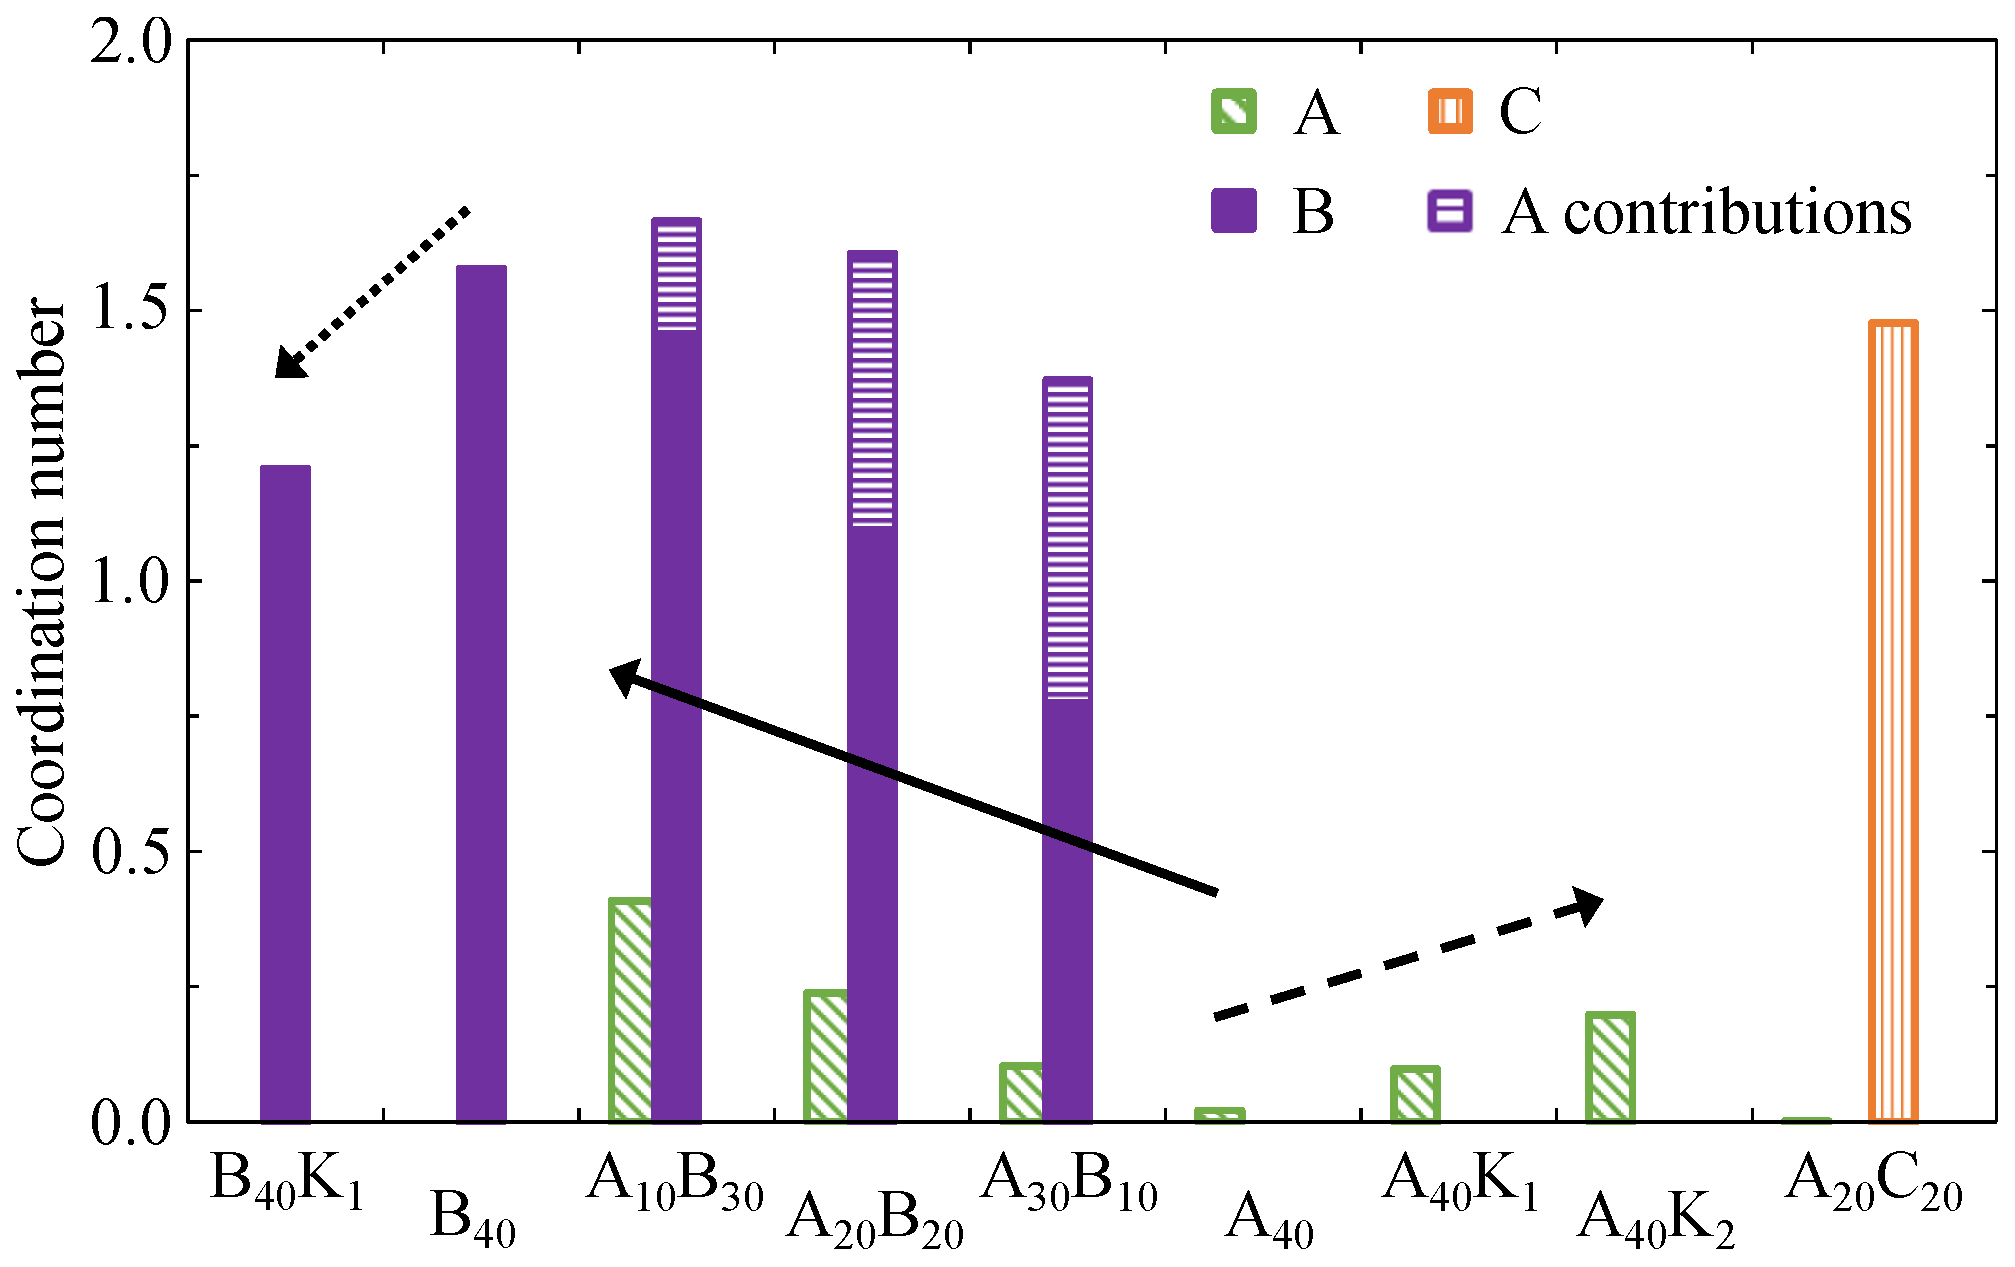
\includegraphics[width=0.8\linewidth]{Figures/CN_bar_chart_updated.eps}
\caption{Molecule-type coordination number values for clusters containing 40 PAHs.}
\label{fig:coordination_numbers}
\end{figure}
% perhaps include cluster snapshots with ribbons to show stacking more clearly?  As insets in bar chart?

We also are interested in which molecule types are present as near neighbours within these heterogeneous systems. We found that the CNs of A have no contribution from A, meaning that all A stacking interactions come from neighbouring B. The majority of B stacking interactions come from other B, however some of the interactions are with A in proportion to the molecular ratios within the cluster, shown as insets with horizontal lines in Fig \ref{fig:coordination_numbers}.
% Contribution of B stacking that came from interactions with A are: two30ann10 12\%, two20ann20 32\%, two10ann30 43\%.

%%% Alignment angles: Molecule sizes have different angles %%% 
Figure~\ref{fig:alignmentangles_homo} presents histograms of the molecular alignment angles, illustrating the relative configurations of neighbouring molecules within the homogeneous clusters studied. It is again immediately clear that the two molecule sizes behave differently but these trends are consistent across all cluster sizes considered (additional cluster size plots can be seen in Figures \ref{fig:alignmentangles_hetero}, \ref{figSI:alignmentangles_cutoffs}, and \ref{figSI:alignmentangles_100}). The systems containing B (top row) show a single significant peak around 20$^{\circ}$.  This suggests that nearly all of the molecules interact in a tilted stack formation, forming 1 dimensional columns in which the molecule bowls possess a concave-to-convex alignment with dipole moment vectors nearly aligned. This small alignment angle provides significant $\pi$-$\pi$ overlap which, within columnar structures, is identified as a feature of materials with good performance in organic electronic devices. This dominant alignment angle is the same that observed between a minimised B dimer (shown as a dashed vertical line), indicating that this is a stable arrangement.  Similar self-assembled structures are observed in crystals containing indenocorannulene molecules \cite{Filatov2010} and other highly curved cPAHs that form polar crystals with strong photoluminescence \cite{chen2014highly}. Neighbouring columnar stacks of B have opposite bowl directions and weak CH-$\pi$ interactions, in which the positively charged rim of one molecule is almost perpendicular to the negative region and the bottom of another molecule in a T-shaped configuration, provide little interaction between columns. Interestingly, the columns show significant tilting at their ends such that parallel columns curve to be nearly continuous, which is not a feature of crystal structures and likely influences cluster surface properties. fPAH clusters also show sharp angle peaks, but these are centred around 0$^{\circ}$ and 180$^{\circ}$, which both correspond to almost perfectly aligned molecular planes (since the alignment angle calculation uses a normal vector), shown in Figure~\ref{figSI:alignmentangles_fPAHs}. This $\pi$-$\pi$ stacking arrangement combines with CH-$\pi$ interactions to produce a herringbone-like structure within both clusters and bulk crystal fPAHs \cite{Khanna200567}, without the column curving present in cPAH clusters.
% corannulene derivatives (with added rings) show significantly improved electrical conductivity compared to the parent corannulene \cite{wang2015electronic} - suggests same for B

In contrast, clusters containing A (bottom row) show a dominant but broad peak around 45$^{\circ}$, with smaller wide peaks around 130$^{\circ}$ and 170$^{\circ}$. 
This agrees with previous work that shows A do not pack with any long-range order \cite{hanson1976crystal,Petrukhina2005,kanao2018differentiating,wang2015electronic,scott1999geodesic} (the angles found in the crystal structure are shown as vertical dashed lines), with some CH-$\pi$ interactions but limited $\pi$-$\pi$ interactions. It is interesting that this bulk molecular arrangement is observed even within the small nanocluster systems examined here. The method constraints of this work highlight that this structure is not due to the rapid bowl inversion dynamics or induced polarities within the system but instead to the molecule size, shape, and electrostatic properties.
% multidimensional analysis shows that the local orientational order of the corannulene molecules are more complex than those of 2pent15ring.  At smaller separation/cut-off distance (< XX nm), the favoured nearest neighbour geometry is XXX (like 45deg angled? vs stacked) while at larger distances (> XX nm) it is XXX (like 90deg??).

%
\begin{figure}[!tbh]
\centering
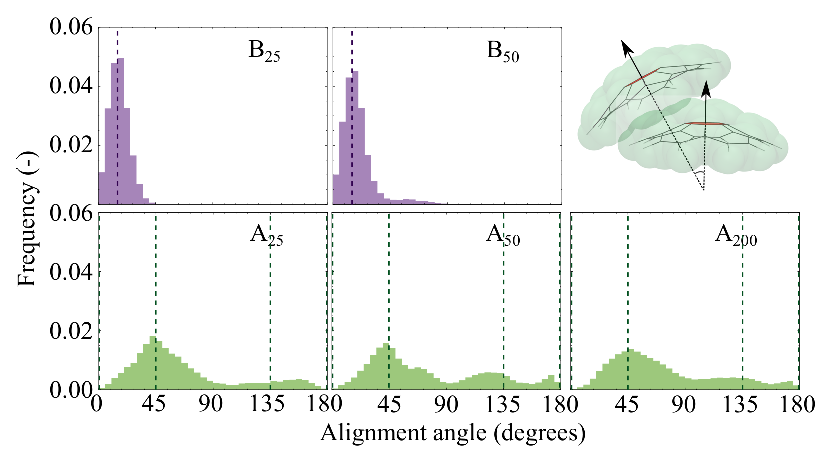
\includegraphics[width=0.84\linewidth]{Figures/alignment_angles_homo.eps}
\caption{Alignment angle distribution for homogeneous B and A clusters across different cluster sizes. A schematic is provided, illustrating an alignment angle of $30^{\circ}$ between two neighbouring A.}
\label{fig:alignmentangles_homo}
\end{figure}
%

Given that the two molecule types self-assemble with different alignment angles, we explore how mixing these molecules influences the alignment angle distributions. Figure~\ref{fig:alignmentangles_hetero} (top row) shows heterogeneous clusters each containing 40 molecules alongside the corresponding homogeneous clusters (middle row). (Additional results from larger clusters are found in the Supplementary Information Section~\ref{figSI:alignmentangles_100}.) In all heterogeneous clusters, the individual molecule alignment peaks align reasonably with those seen in the homogeneous clusters, A crystal structure, and B dimer, with the majority of B around 20$^{\circ}$ and many A around 45$^{\circ}$. There is an additional small B peak around 45$^{\circ}$, indicating some deviations from columnar stacking that align with the dominant arrangement of A. This is more pronounced in clusters containing $ge$50\% A, suggesting that A molecules are located within B columns. The molecule proportions also influence A angles, with shifts towards lower angles and loss of values around 130$^{\circ}$. The $\text{A}_{\text{30}}\text{B}_{\text{10}}$ cluster shows a distribution similar to that of the homogeneous A cluster, although the peaks are much broader. As the proportion of B increases their influence is felt on A so that in the equi-ratioed cluster ($\text{A}_{\text{20}}\text{B}_{\text{20}}$), the A peak at 45$^{\circ}$ is spread out towards 0$^{\circ}$ and the former 135$^{\circ}$ peak is pushed towards 170$^{\circ}$. In the cluster containing 75\% B ($\text{A}_{\text{10}}\text{B}_{\text{30}}$), the largest angle peak for A aligns with that of B at 20$^{\circ}$. This indicates that A are stacking in a similar fashion to B, which can be seen in the cluster snapshot (Figure~\ref{fig:clustersnapshots}) where A predominantly interact individually at the ends of B stacks, fitting in the concave or convex surfaces. Although similar molecule size interactions are observed in heterogeneous fPAH clusters, these planar aromatics do not self-assemble with different alignments depending on molecule size and thus heterogeneous clusters show the same highly aligned columnar stacking behaviour as homogeneous clusters, as shown in Figure~\ref{figSI:alignmentangles_fPAHs}.
%
\begin{figure}[!tbh]
\centering
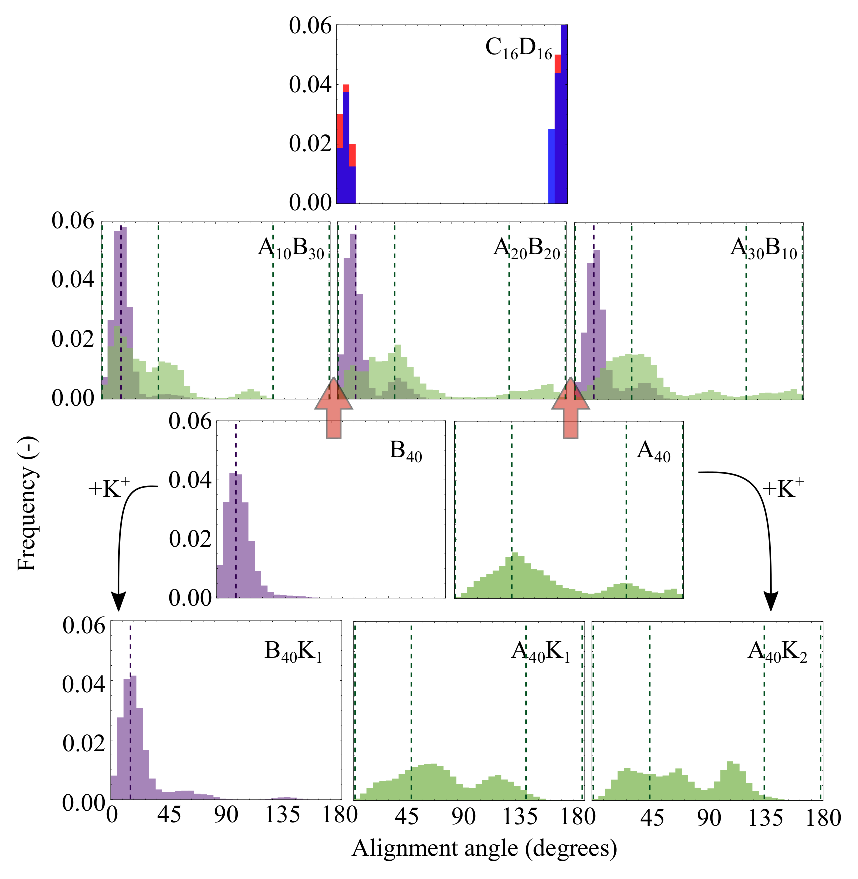
\includegraphics[width=0.85\linewidth]{Figures/alignment_angles_hetero.eps}
\caption{Alignment angle distributions for A and B clusters containing 40 molecules. The middle row shows the homogeneous clusters, with red arrows showing the heterogeneous clusters (top row) and curved arrows indicating ion-containing clusters (bottom row).}
\label{fig:alignmentangles_hetero}
\end{figure}
%

This detailed evaluation of intermolecular spacing, CNs, and alignment angles shows that the self-assembly of cPAHs depends strongly on their size and not the cluster size. Strong CH-$\pi$ attractions between molecule rims and bowl centres control the arrangement of A while dipole-dipole attractions and dispersive surface interactions produce B structures. This molecule size dependent structure is observed within the crystal structures of cPAHs and also influences the behaviour of heterogeneous systems. Systems containing B show high CNs and low angles, suggesting good molecular alignment like fPAHs. However, clusters containing even small proportions of A disrupt mesophase formation.
% curvature disrupts mesophase formation, particularly when mixtures of cPAHs are present.

% To add in somewhere?: Understanding the stacking behaviour of curved PAHs is relevant to materials studies / supramolecular chemistry / crystalline organic materials ( relevant to polymers of intrinsic microporosity, graphene systems, graphene quantum dots (experimental condensation structure)) because of their unique optical and conduction properties; and can also lead to using these molecules as building blocks for engineering organic crystals with desired properties.  

%%%%%%%%%%%%%%%%%%%%%%%%%%%%%%%%%%%%%%%%%%%%%%%%%%%%%
%%%% Question 2: What is the internal structure? %%%%
%%%%%%%%%%%%%%%%%%%%%%%%%%%%%%%%%%%%%%%%%%%%%%%%%%%%%
% Do cPAH self-assemble into core-shell nanoparticles?
\subsection{What is the internal structure of cPAH clusters?}
Characterising the internal nanostructure of cPAH clusters provides valuable information relevant to the formation and composition of combustion-generated nanoparticles as well as the design of nanoparticles for optoelectronic applications. In this section we will discuss cluster densities and energies and will use radial distances to consider the partitioning behaviour of clusters containing different ratios of molecule sizes.

%% diameters and densities
Cluster diameters and densities show that cPAHs form tightly packed clusters. Homogeneous B clusters possess densities of 1.52--1.59 g/$\text{cm}^{3}$, which is comparable to mature graphitised soot particles (1.50--2.08 g/$\text{cm}^{3}$ \cite{johansson2017evolution}) although still lower than graphite (2.09--2.23 g/$\text{cm}^{3}$). A cluster densities are between 1.45 and 1.50 g/$\text{cm}^{3}$, higher than that of the A crystal structure (1.36 g/$\text{cm}^{3}$ \cite{Petrukhina2005}) and comparably sized fPAH clusters (1.39--1.46 g/$\text{cm}^{3}$ \cite{chen2014size}) but still within the range ascribed to young soot particles (1.12--1.50 g/$\text{cm}^{3}$ \cite{totton2010modelling,camacho2015mobility}). All cluster densities decrease with increasing cluster size, although this effect is muted for cPAH clusters compared to their fPAH counterparts. The diameter and density values of heterogeneous cPAH clusters are consistent with simple mixing averages of the analogous homogeneous cPAH clusters, suggesting that heterogeneity does not cause a dramatic change in the overall cluster shape and packing, although further analysis will examine internal and molecule-specific effects.

%%% Core-shell type partitioning of molecule sizes - not as distinct as fPAHs and not dependent on cluster size or molecular ratio %%%
We are particularly interested in whether cPAHs show the same core-shell partitioning seen in fPAH systems, where the cluster core consists of the larger fPAHs and the shell contains the smaller fPAHs \cite{bowal2018partitioning}. Average radial distances between each molecule type and the cluster centre are calculated to provide an indication of the molecule-type positioning within each cluster, tabulated in  Table~\ref{table:maintable}. For the homogeneous cases, the two molecule types show similar relative average radial distances at 75--85\% (76--86) of the total cluster radius, similar to the fPAH clusters (for example, $\text{C}_{\text{100}}$ has a value of 77\% \cite{chen2014size}). However, in all clusters containing two molecule types A possess larger average radial distances (located within 80--90\% of the total cluster radius) than the B (70--80\% of the cluster radius). This is indicative of a core-shell structure in which the larger molecules reside in the cluster core, as seen in fPAH clusters (for example, the average radial distances of C and D are 89\% and 65\% of the cluster radius, respectively, for $\text{C}_{\text{16}}\text{D}_{\text{16}}$ \cite{bowal2018partitioning}).

Although the average radial distances show a core-shell partitioning of molecule sizes, the equilibrium distribution of radial distances shows that this radial separation is less distinct for clusters containing cPAHs compared to similar fPAH clusters. Figure~\ref{fig:radialdists_atomic} shows that there is significant mixing of the molecule types within the cPAH clusters and molecules of both types present near the cluster centre, regardless of cluster size or molecular ratio.
%
\begin{figure}[!tbh]
\centering
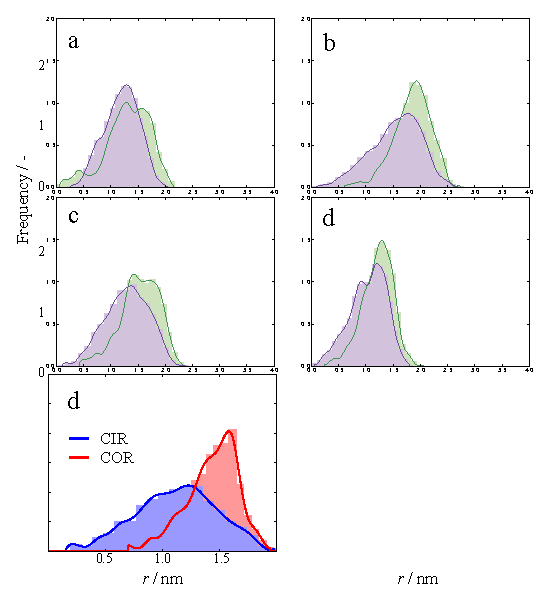
\includegraphics[width=0.6\linewidth]{Figures/radii_histograms_aa.eps}
\caption{Normalised atomic radial distance distributions for heterogeneous PAH clusters. The fPAH cluster $\text{C}_{\text{16}}\text{D}_{\text{16}}$ is obtained from \citet{bowal2018partitioning}.}
\label{fig:radialdists_atomic}
\end{figure}
%

We have previously explored the contribution of flexoelectrically polarised aromatics to soot formation \cite{Martin2018flexo} and it follows that long-range dipole-dipole interactions between cPAHs may allow cPAH clusters to possess increased stability compared to fPAHs.  This would have particular interest to contexts in which stable PAH nanoparticles are present, such as combustion and interstellar medium.  To address this hypothesis, we present intermolecular energies as a function of mass for cPAH and fPAH clusters, shown in Figure~\ref{fig:energies}.  The energies are shown per atom in the system, in order to facilitate direct comparison between systems of different cluster and molecule sizes. It is clear that in all cases the energy decreases with cluster mass. Homogeneous clusters containing fPAHs (all coloured similarly here to allow for ease in reading), taken from \citet{chen2014size,chen2015solid}, show relatively consistent energy trends across molecule sizes from pyrene to circumcoronene, with heterogeneous clusters, taken from \citet{bowal2018partitioning}, generally at lower energy values. Clusters containing cPAHs tend to have lower energies than fPAHs, as predicted based on their increased electrostatic attraction, although this is dependent on cPAH cluster composition. Clusters containing B show energies similar to those of heterogeneous fPAH clusters and A clusters possess lower mass-weighted energies.
%
\begin{figure}[!tbh]
\centering
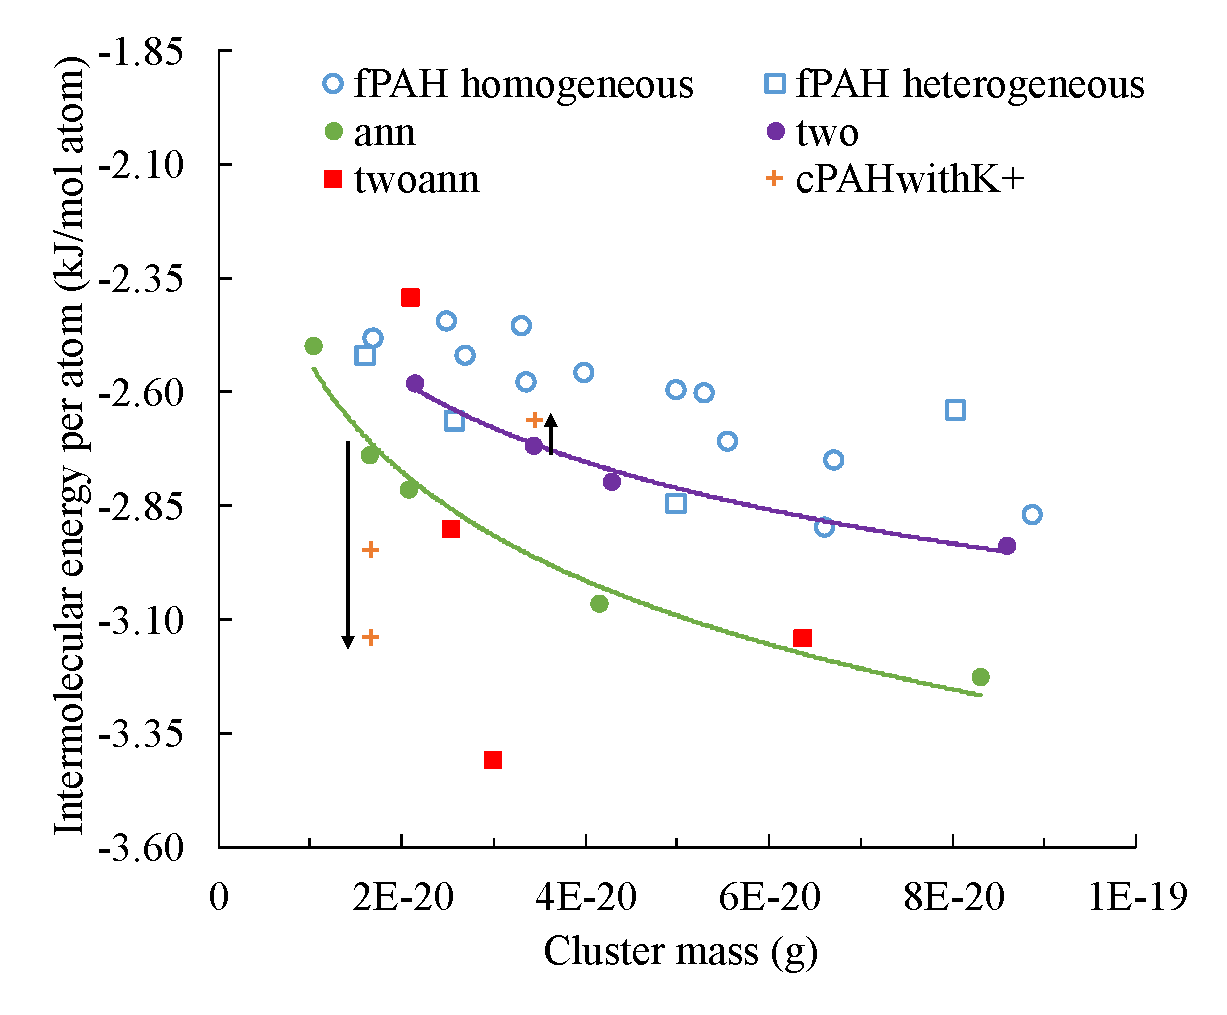
\includegraphics[width=0.8\linewidth]{Figures/energies.eps}
\caption{Intermolecular energy per atom versus cluster mass for all clusters considered in this work. Lines are drawn for the cPAH homogeneous clusters to guide the eye and black arrows show the energy changes caused by the addition of a cation(s). The subscript y is used to denote an unspecified number of molecules in order to consider multiple clusters.}
\label{fig:energies}
\end{figure}
% make f/cPAH cluster point orange to match colouring?  Change red points to avoid confusion with C? - can make those black!

The effect of heterogeneity in cPAH clusters shows a distinct effect of molecular ratio: an increased proportion of B in the cluster decreases the energy. At a equi-molecule ratio, the heterogeneous cluster energies reflect that of homogeneous A clusters across cluster sizes. However, changing the molecule proportions affects the cluster energies significantly: $\text{A}_{\text{30}}\text{B}_{\text{10}}$ possesses a high energy while $\text{A}_{\text{10}}\text{B}_{\text{30}}$ has a low energy, producing the highest and lowest energy clusters of all the ones we evaluate here. This suggests that in all cases the presence of B increases cluster stability if above 50\% composition.

These energy trends are in agreement with the structural metrics discussed previously, so that a higher degree of order within the hetergeneous cPAH clusters (increased stack formation as quantified by CNs, for example) corresponds to a greater interaction strength. This highlights that the stacking of A within the bowls of B increases the cluster intermolecular energy until a proportion (<50\% A) at which the presence of A disrupts B stacking by inserting within columns instead of only residing at column ends, thereby destabilising the cluster.
% TO DO: add summary statement to answer question

%%%%%%%%%%%%%%%%%%%%%%%%%%%%%%%%%%%%%%%%%%%%%%%%%%%%%
%%%% Section 3: complex cPAH clusters %%%%%%%%%%%%%%%
%%%%%%%%%%%%%%%%%%%%%%%%%%%%%%%%%%%%%%%%%%%%%%%%%%%%%
\subsection{How do cPAH clusters containing fPAHs or ions self-assemble?}

Many practical applications involve systems that contain many molecule types. Of particular interest to combustion and material scientists are cPAH systems that also contain fPAHs or ions. We investigate relevant representative clusters using all of the metrics previously discussed to show the influence of different molecule curvatures and ion interactions within cPAH systems.

\subsubsection{Particles containing cPAHs and fPAHs}
To evaluate the self-assembly of clusters containing curved and flat PAHs, we consider $\text{A}_{\text{20}}\text{C}_{\text{20}}$. This cluster shows a distinct partitioning of the molecule types in a janus configuration, in contrast to the mixed arrangement seen in homogeneous clusters and the core-shell structure seen in heterogeneous clusters containing either fPAHs or cPAHs. The average intermolecular spacing of 0.43~nm comes almost entirely from neighbouring C, and matches the spacing calculated for a homogeneous C cluster \cite{chen2014phase}). This suggests that the fPAH molecules orient in a stacked configuration, but the constituent cPAHs do not. This is highlighted in a detailed CN evaluation which shows constituent C have a CN of approximately 1.5 while A have no near neighbours within a stacked configuration cut-off radius (CN of 0.0). These values agree with the respective homogeneous C and A clusters, as do the molecular alignment angles (Figure~\ref{figSI:alignmentangles_ann20cor20}). These distinct types of local ordering cause the mixed fPAH and cPAH cluster to produce a janus particle with two different halves, highlighted by similar molecule-type radial distances (Table~\ref{table:maintable}). This cluster containing both curved and flat PAHs has an energy similar to that of homogeneous cPAH clusters, indicating that the mixing of molecule types does not enhance molecule interaction energy and instead it remains similar to that of the weaker component.

Dispersion and electrostatic interactions dominate the attractive forces between homogeneous interactions of fPAHs and cPAHs. However, this mixed molecule system is hindered by sterics and mismatched polarities and thus produces weaker interactions and a relatively low density. In this way the stronger interactions between like molecules contribute to a particle system in which the two molecule types are immiscible. Many material systems, such as coal and soot particles are seen experimentally to possess both curved and flat aromatics. These results suggest that when molecule-type separation is not observed in such systems, self-assembly through physical interactions does not control the molecular structure. For example, covalent bonding between fPAHs and cPAHs may explain why soot particles do not form janus particles.
%
%Relate these clusters and their properties to experimental structures (potential implications for synthesis, potential applications, etc).
% relevant to formation / nature of janus particles, for example ones that are polar on one side
% do not experience any enhancement in electrostatic interactions (in a non-polarisable potential description). not including some advanced interactions such as induced dipoles

\subsubsection{Particles containing cPAHs and ion(s)} 
% How do cPAH self-assemble around ions?

% TO DO: add in this "Previous work has characterised the first solvation shells of fPAH molecules around an alkali-metal ion (Bartolomei, Bowal, Dongping?), but this has not been explored allowed for the characterization of the first solvation shells of cPAH molecules of coronene around an alkali-metal ion" (

%%% ions change the structure of cPAH clusters different depending on molecule size %%%
We further explore the influence of heterogeneity by considering clusters containing 40 molecules (A or B) and one or two potassium cations.  These systems can be directly compared to homogeneous systems of the same size. Potassium ions are selected because they are known to interact with cPAHs in systems of interest (refs - combustion/production) and because the intermolecular interactions between this cation and cPAHs have already been parameterised with the curPAHIP potential \cite{bowal2019ion}. As seen in Table~\ref{table:maintable},
the inclusion of ion(s) within the cPAH clusters appears to increase the cluster diameter, and thus decrease the cluster density, slightly.

%\subsubsection{Intermolecular spacing and stacking}
Intermolecular spacing values also change slightly with the addition of a cation(s). The B cluster experiences a small increase in the spacing, while the A clusters show an increase and decrease in the spacing values depending on the number of cations present. This suggests that the cation has an effect on molecular arrangement, although in opposite ways depending on the constituent cPAH size. % differences maybe not big enough to make these statements?!  Shorten this paragraph (already mostly combined below)

CNs for ion-containing clusters complement the intermolecular spacing results. The B cluster CN decreases with the addition of \ce{K+}, suggesting a disruption of the highly stacked ordering in agreement with an increased intermolecular spacing. Conversely, the A clusters show increased ordering with higher CNs and also decreased average spacing. This effect increases with the addition of a second cation, although the CNs are still significantly lower than those of the B clusters.

%\subsubsection{Radial distances}
The addition of a potassium cation(s) also results in slightly %(2-3\%)
decreased radial distances for both molecule types, so that average molecular distance values are around 75\% of the total cluster radius. The average radial distance decreases with the addition of a second cation. %% not significant enough??
This suggests that the cation influence is additive, although further work needs to be done to assess when this trend reaches a saturation level or perhaps has cancelling or negative effects. 

% TO DO: add summary statement to answer question

%%% to include?
%Radial distance histograms show that introducing \ce{K+} into cPAH clusters produces an increase of cPAH molecules with very small radial distance values, suggesting that the ion(s) promotes an increased molecular ordering at/around the cluster centre. This is more marked for the B cluster case than A. % add or reference corresponding figure(s)? note that this is visible in homo cPAH molecular radial distance histograms not show... see log notes.  Perhaps include these plots - can overlay histograms to show effect.  Can show ion position(s) with dashed lines in these plots.  And this could segue into talking about how the ion(s) influence the molecular structure around them...
% The radial position of the ion(s) within the cluster does not correspond to a clear grouping/structure of cPAH molecules. 
% Therefore, although the presence of an ion(s) causes more cPAH molecules to order around the cluster centre, this does effect seems to be very local and the total cluster shape/size is not changed very much.

%\subsubsection{Alignment angles}
The alignment angle distributions, seen in Figure~\ref{fig:alignmentangles_hetero}, of A clusters containing \ce{K+} are different than the homogeneous case and the crystal structure, with a broadening and splitting of the 45$^{\circ}$ peak, increase in the 120$^{\circ}$ peak, and disappearance of high angles (around 170$^{\circ}$). The alignment angles of B also change with the addition of a cation, with a broadened distribution around 20$^{\circ}$ and additional angles present around 55$^{\circ}$ and 135$^{\circ}$. This shows that the addition of a cation disrupts the stacked structure otherwise seen in homogeneous or heterogeneous clusters containing B. 
% It is interesting to note that the number of neighbouring molecules within the cut-off distance decreased for 2pent15ring molecule systems with the addition of a potassium cation. (this is seen in comparing cut-off distances behaviour) - is this still true after recalculating?

%\subsubsection{Energies}
%%% ann clusters have lower mass-weighted energy than 2pent15ring, addition of some corannulene decreases energy (50/50 gives same as ann), fPAHs have higher energies %%%
The presence of cation(s) in the cluster has opposite effects on clusters containing the two molecule types: B clusters with \ce{K+} show an increased energy, while clusters with A containing \ce{K+} showed a decreased energy in proportion with the number of ions.  These differences are shown with black arrows in Figure~\ref{fig:energies}. This suggests that the ion influences molecular interactions and cluster structure in different ways depending on the molecule size, in agreement with the structural metrics evaluated.

These quantitative differences suggest that the addition of a cation promotes stacking within the A cluster and disrupts the existing stacking within the B cluster. This can be observed in the cluster visualisations in Figure~\ref{fig:clustersnapshots}, which highlight the atoms immediately around the cation(s). All clusters show a solvation shell of 4 molecules around each cation with the cPAH electron-rich convex surfaces face towards the cation(s). A form a tetrahedral-like formation, called a "flower`` motif in \citet{bowal2019ion}, compared to the a staggered triangular "propeller`` motif adopted by fPAHs around a cation \cite{bartolomei2019aggregation}. The formation of a solvation shell serves to provide a seed for A structure while disrupting the long B stacks.

\section{Conclusions}
Curved carbons are ubiquitous and have great promise in many systems and applications such as particulates, novel nanocarbon materials, and sensors. This work provides a first detailed exploration of the nanostructure of particles containing cPAHs, examining their structure in homogeneous clusters containing one molecule type only, heterogeneous clusters containing different cPAH sizes and ratios, and cPAH clusters containing fPAHs or cations.

The previously developed curPAHIP potential was extended to capture the interactions between large cPAHs and mixed cPAH systems. Structural metrics, including intermolecular spacing, coordination number, and alignment angles show that the nanostructure of homogeneous cPAH particles is dependent on molecule size but unaffected by particle size (from 2 - 5 nm). B form parallel stacks whereas A do not possess short-range order, although both particle systems show similarities to the crystal structures of comparable cPAHs.

Mixing of cPAH sizes influences particle structure. The addition of A to a particle containing B serves to enhance the $\pi$-$\pi$ stacking and interactions of A, resulting in lower energy particles. %Both the CN and energy values suggest that B clusters with some added (<50\%) A are the most stacked and stable.
Regardless of molecular ratio, heterogeneous cPAH particles show a core-shell type arrangement similar to but less distinct than the partitioning observed in fPAH particles. Particles containing fPAHs and cPAHs self-assemble into janus particles, with minimal interaction between the molecule types, suggesting that the two molecule types are not miscible. Further work to thoroughly develop a fPAH-cPAH intermolecular potential and test the effect of molecular composition should be done to further explore the formation of semi-polar janus particles containing cPAHs and fPAHs. 

The addition of cations to cPAH particles causes the formation of a solvation shell which influences the internal particle structure. A show enhanced local order, while the stacked structure of B is disrupted due to the cations present. Further work should examine the influence of ion charge, size, and number on these structural properties. Future work should also consider the presence of additional atoms within cPAHs, since the interactions between curved aromatic molecules containing heteroatoms, such as oxygen, show increased dimer interactions that provide further electrostatic stabilisation \cite{Cabaleiro-Lago2018}.  


\section*{Acknowledgements}
This work used the ARCHER UK National Supercomputing Service (\url{http://www.archer.ac.uk}).
K.B. is grateful to the Cambridge Trust and King's College, Cambridge for their financial support.
This project is also supported by the National Research Foundation (NRF), Prime Minister's Office, Singapore under its Campus for Research Excellence and Technological Enterprise (CREATE) programme.
